\newpage
\begin{appendix}
\section{Anhang}
Folgende Dokumente befinden sich in schriftlicher Form im Anhang:

\begin{itemize}
	\item \verb|Projektplan Maschinentechnik|
	\item \verb|Projektplan Elektrotechnik|	
	\item \verb|Risikomanagement|
	\item \verb|Pflichtenheft v1.6|	
	\item \verb|Funktionsbezogene Variation|
	\item \verb|Morphologischer Kasten|	
	\item \verb|Berechnungen Spindel|
	\item \verb|Schema Mainboard PCB|
	\item \verb|Schema Baseboard PCB|	
\end{itemize}

Folgende Dateien befinden sich in digitaler Form im Anhang:

\begin{itemize}
	\item \verb|Aufgabenstellungen und Projektskizzen|
	\item \verb|Berechnungen|
	\item \verb|Datenblätter|
	\begin{itemize}
		\item \verb|Elektrotechnik|
		\item \verb|Maschinentechnik|
		\item Datenblatt Ricoter Gartenhumus.pdf
		\item Datenblatt Töpfe - VCD Pöppelmann.pdf
		\item Datenblatt Topfkranz TC2.pdf
	\end{itemize}	
	\item \verb|Fertigungsunterlagen|
	\begin{itemize}
		\item \verb|Additive Fertigung|
		\item \verb|Lasertrennverfahren|
		\item \verb|Spanende Bearbeitung|
	\end{itemize}	
	\item \verb|Finanzierung|
	\begin{itemize}
		\item \verb|Budget HSLU|
		\item \verb|erste Offerte|
		\item \verb|zweite Offerte|
		\item Übersicht Gesamtabrechnung.pdf
	\end{itemize}
	\item \verb|Konstruktion|
	\begin{itemize}
		\item \verb|_parts library|
		\item \verb|Funktionsnachweise|
		\item \verb|HMI|
		\item \verb|Setzeinheit|
		\item \verb|Stechdorn|
		\item \verb|System|
		\item \verb|Testumgebung|
		\item \verb|Vereinzelung|
		\item \verb|Verstellmechanik light M12|
	\end{itemize}
	\item \verb|Konzept|
	\begin{itemize}
		\item \verb|Mindmaps|
		\item Funktionsbezogene Variation.pdf
		\item Morphologischer Kasten.pdf
	\end{itemize}
	\item \verb|PCBs|
	\begin{itemize}
	\item \verb|Baseboard_TMCM-1630_PCB|
	\item \verb|HMI_LED_PCB|
	\item \verb|Mainboard_PCB|
	\end{itemize}
	\item \verb|Software FRDM-Board|
	\item \verb|Verdrahtung|
	\item Pflichtenheft v1.6.pdf
	\item Projektplan Elektrotechnik.pdf
	\item Projektplan Maschinentechnik.pdf
	\item Risikomanagement.pdf
\end{itemize}

%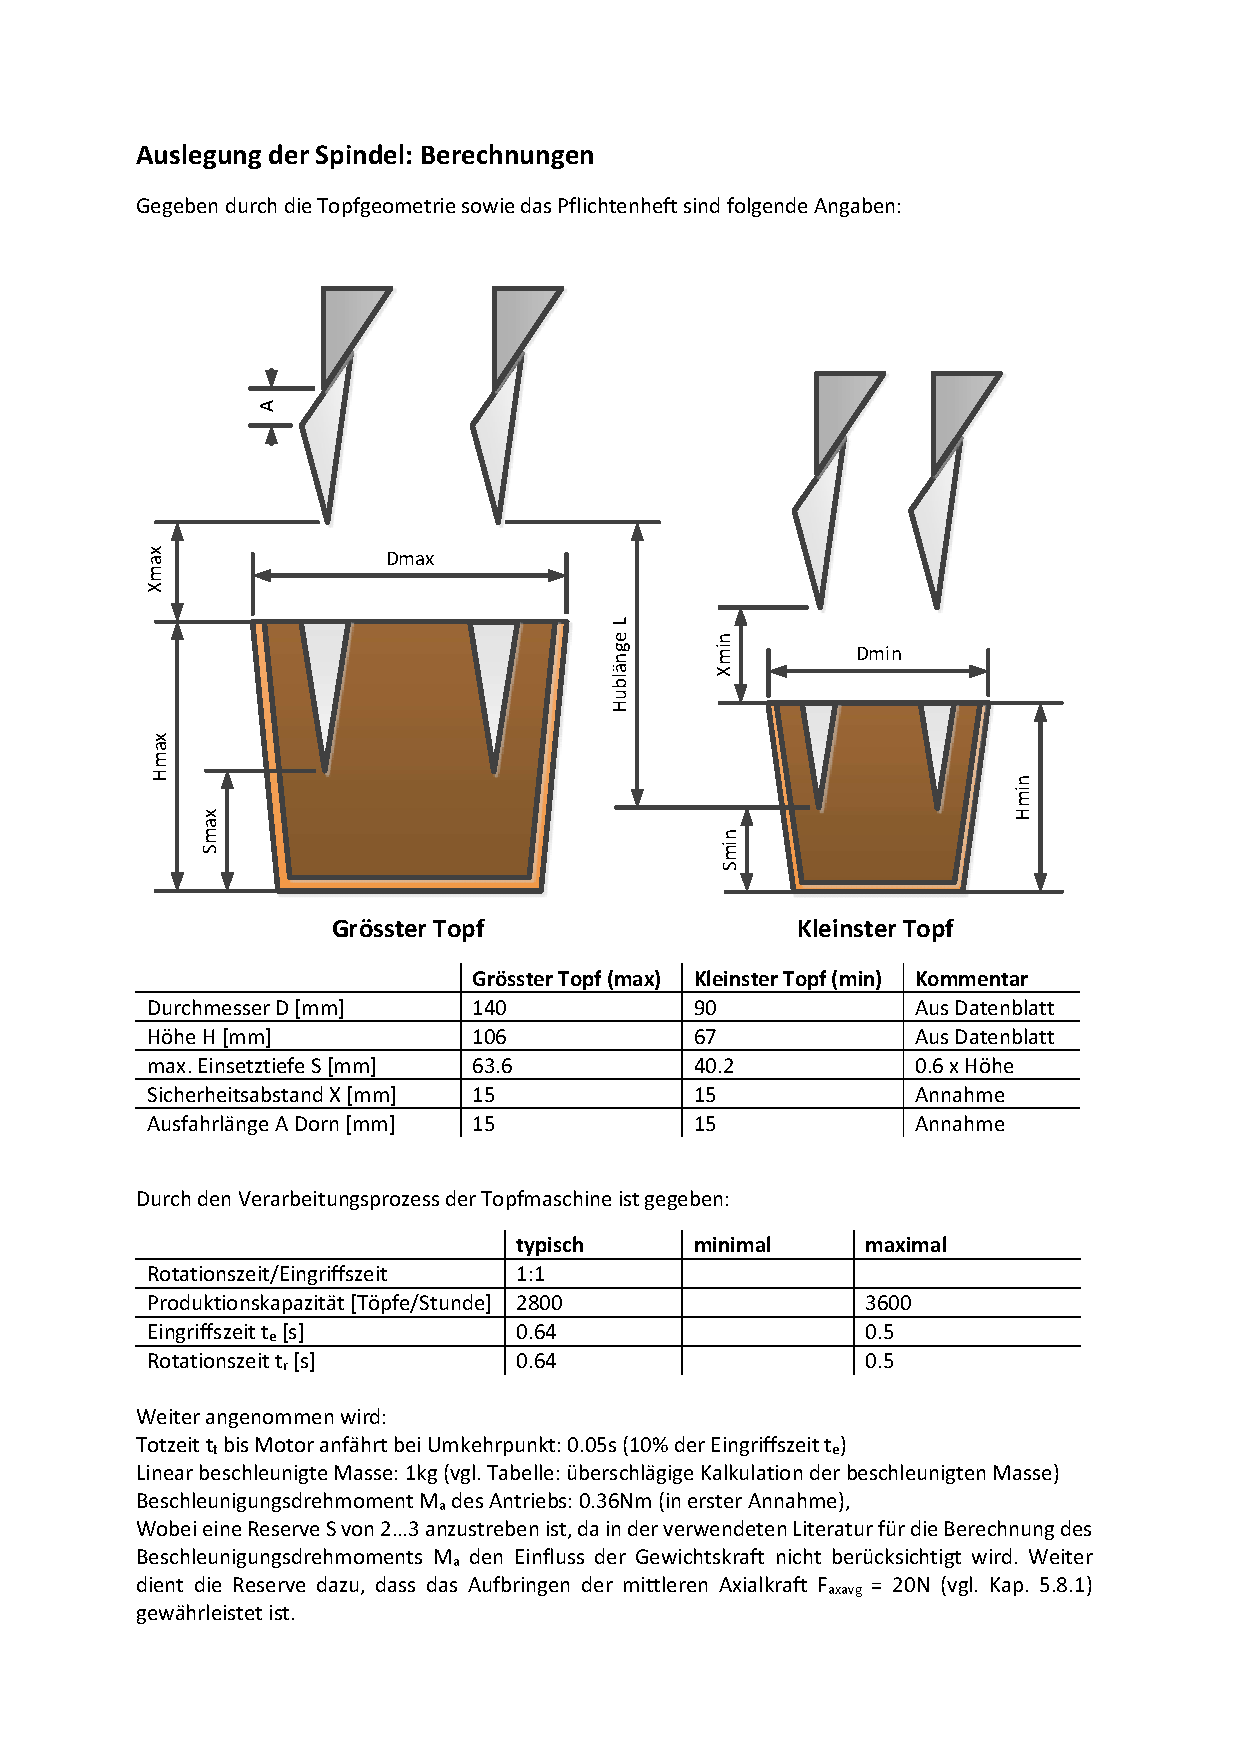
\includepdf[pages=-,nup=1x1]{Illustrationen/10-Anhang/Auslegung Spindel.pdf}
%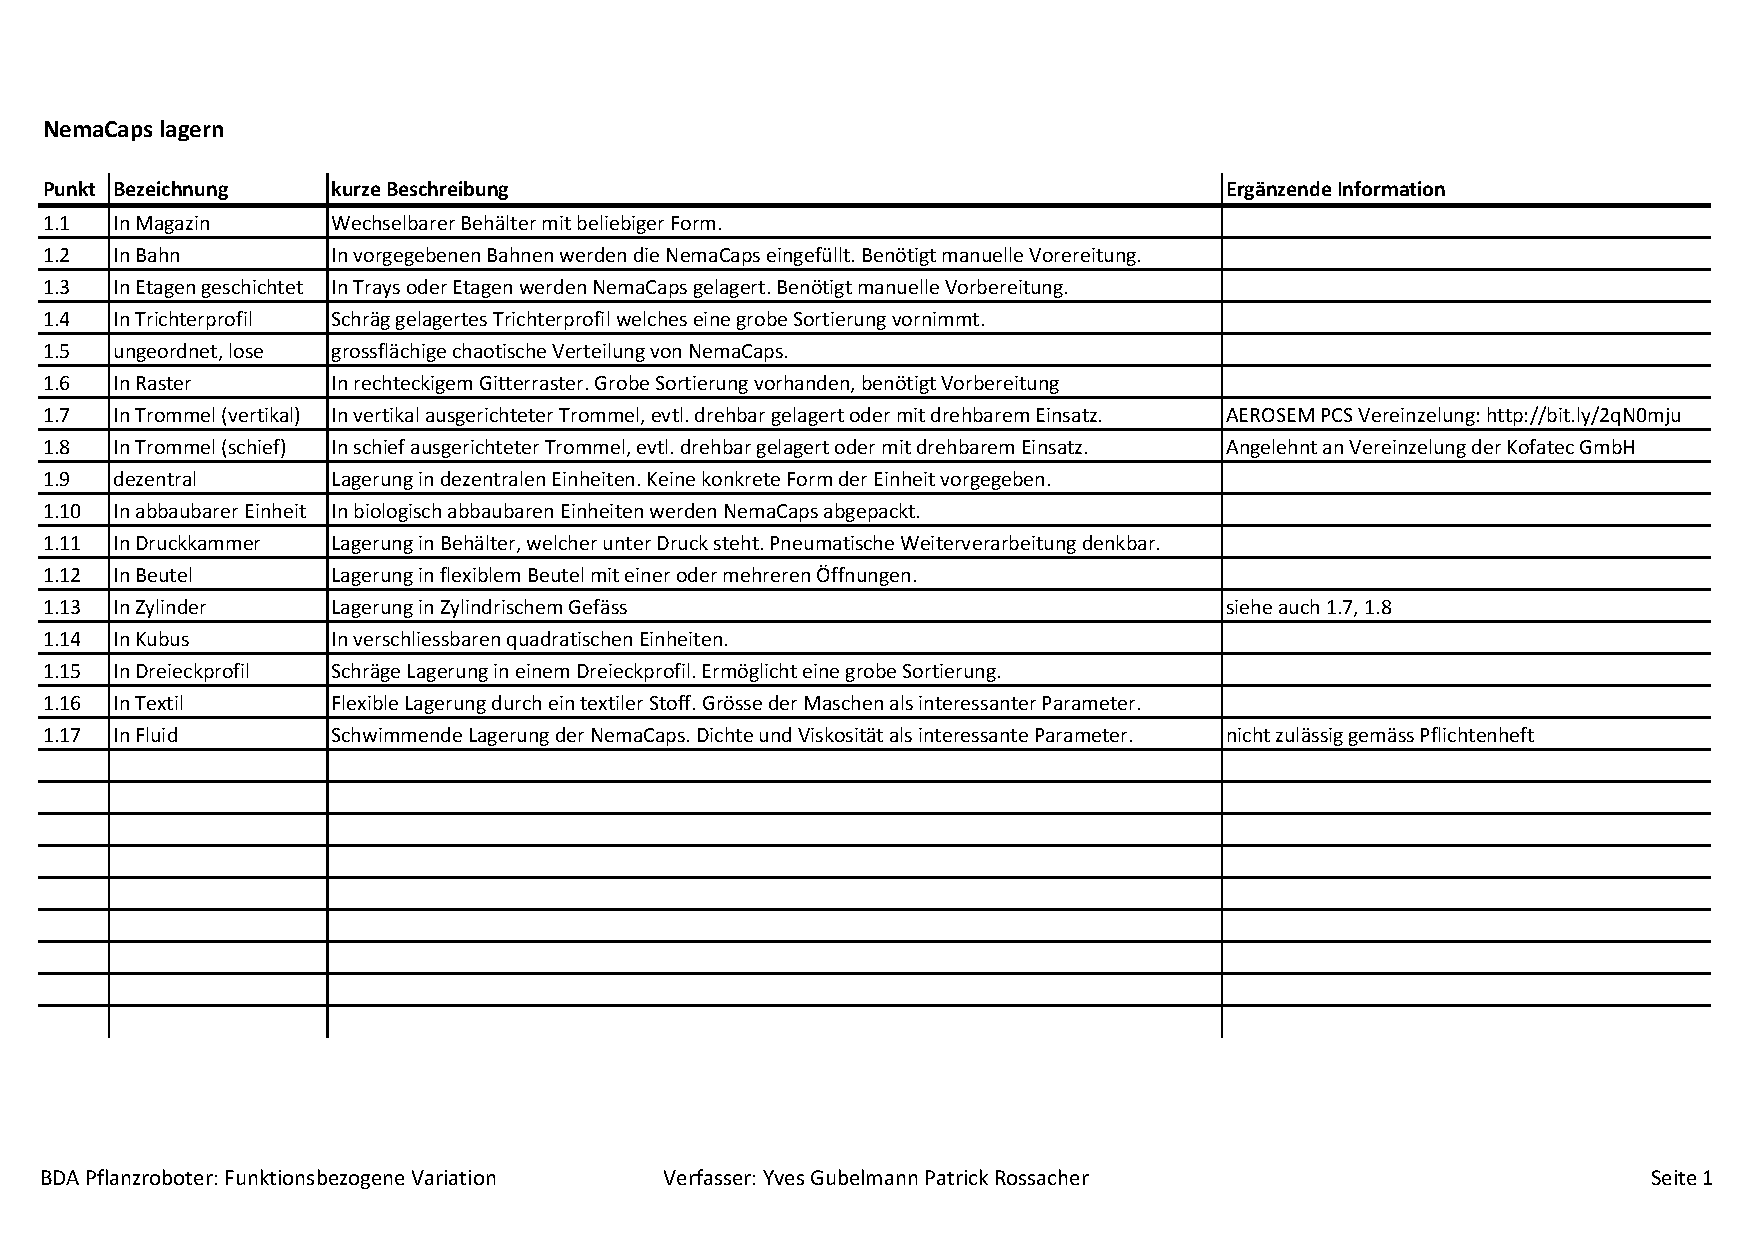
\includepdf[pages=-,nup=1x1]{Illustrationen/10-Anhang/Funktionsbezogene Variation.pdf}
%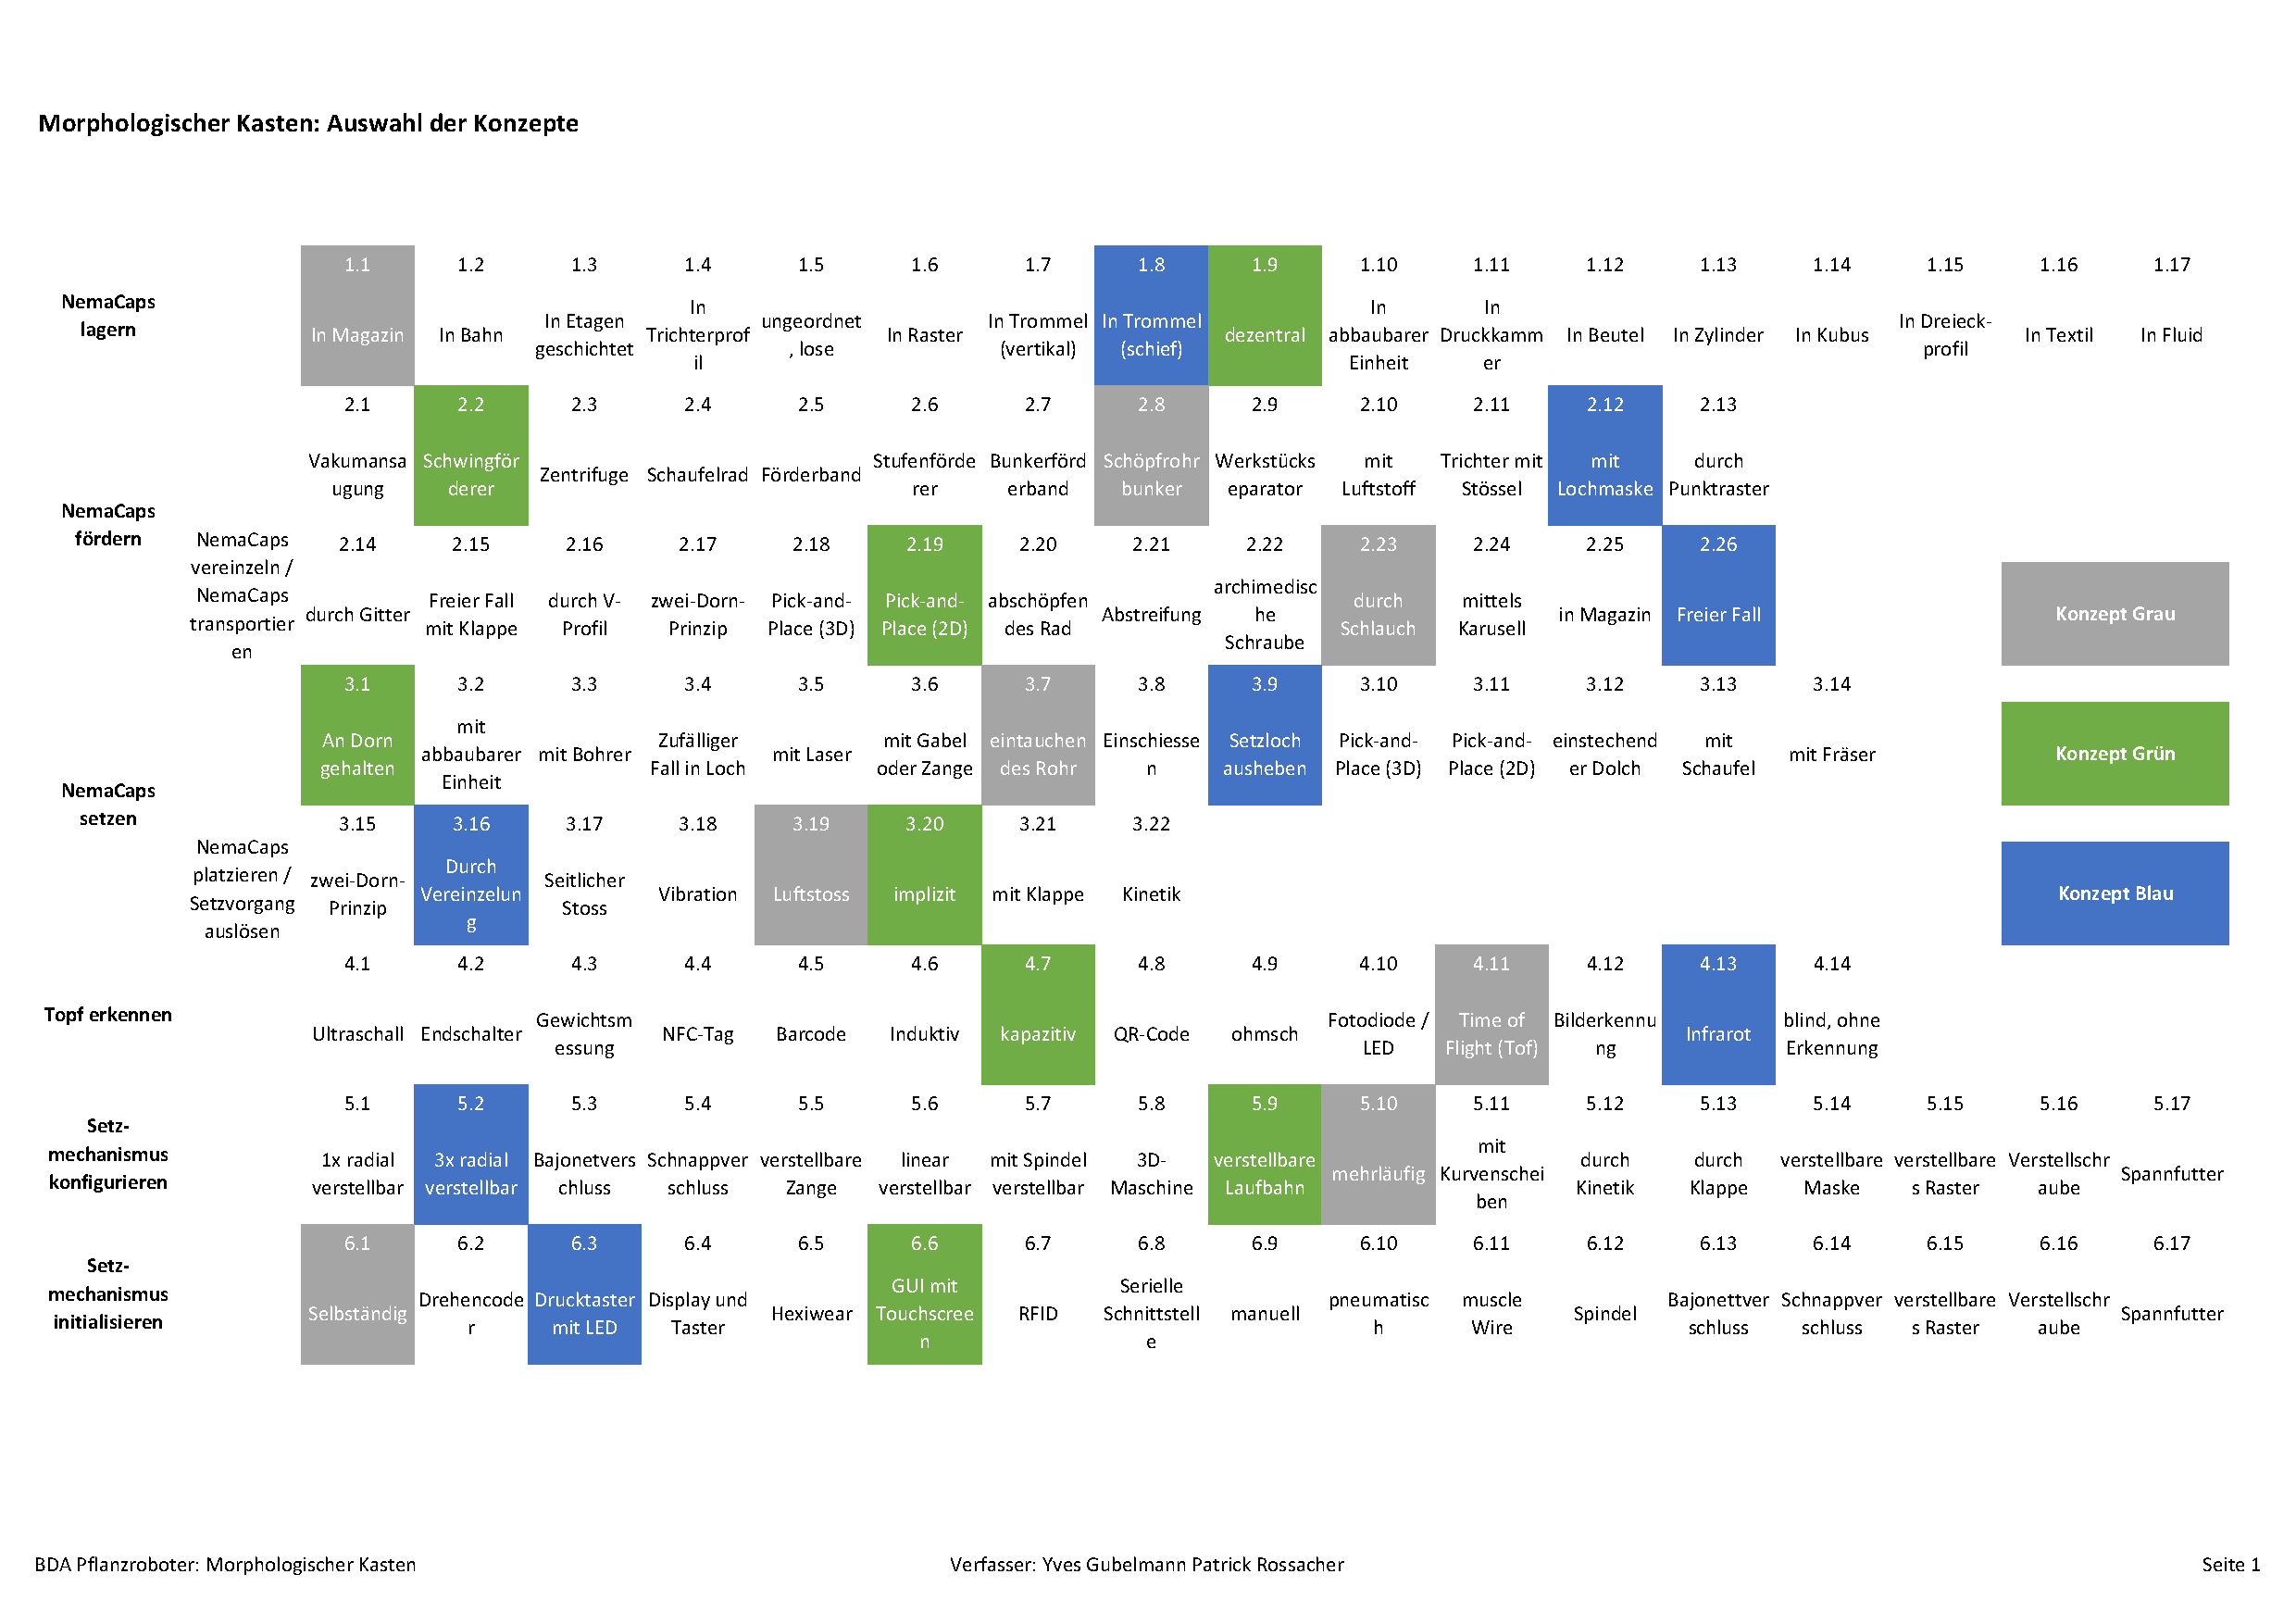
\includepdf[pages=-,nup=1x1]{Illustrationen/10-Anhang/Morphologischer Kasten.pdf}
%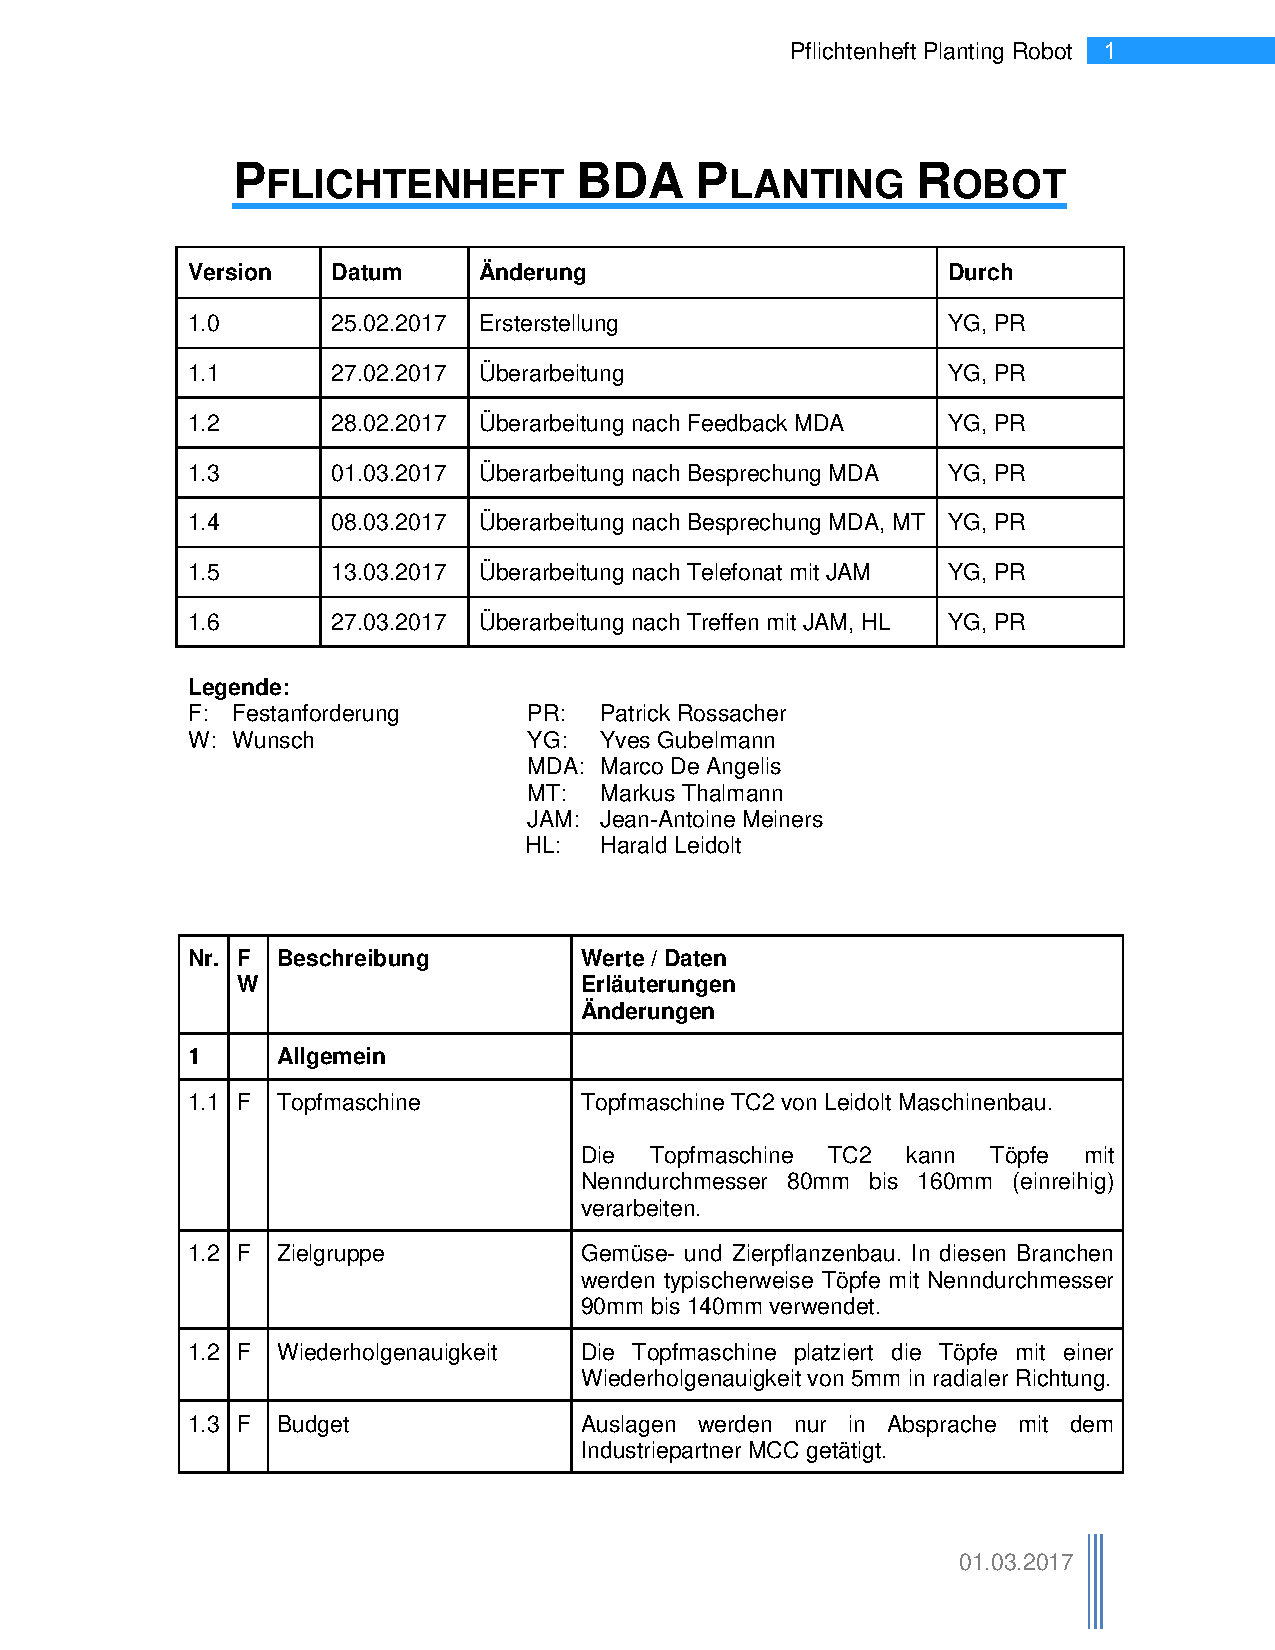
\includepdf[pages=-,nup=1x1]{Illustrationen/10-Anhang/Pflichtenheft v1.6.pdf}
%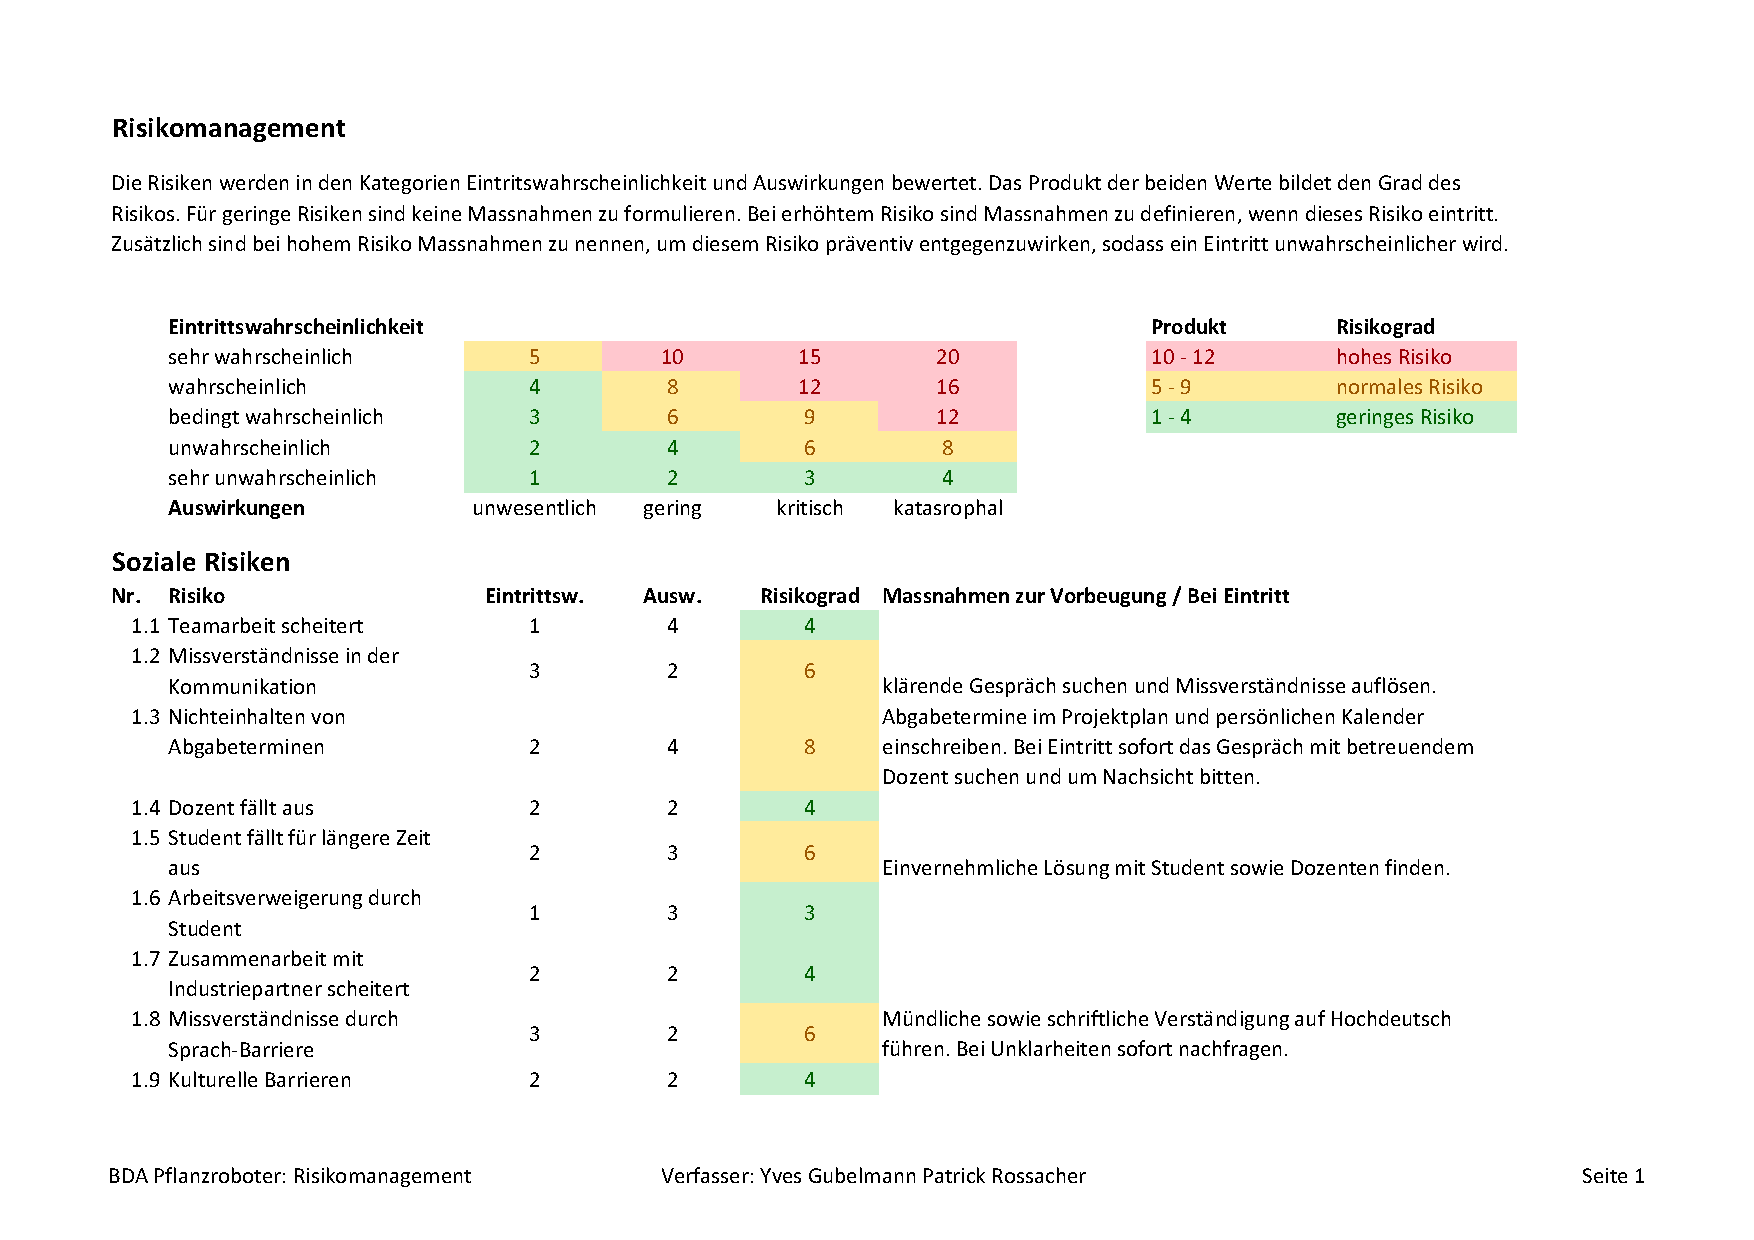
\includepdf[pages=-,nup=1x1]{Illustrationen/10-Anhang/Risikomanagement.pdf}

\end{appendix}